% TikZ libraries for drawing shapes, arrows, and positioning
\usetikzlibrary{
    arrows.meta,
    backgrounds,
    calc,
    matrix,
    positioning,
    shapes.geometric
}

% Define colors used in the SVG diagram
\definecolor{bggray}{HTML}{f8f9fa}
\definecolor{darkblue}{HTML}{2c3e50}
\definecolor{lightbluefill}{HTML}{e3f2fd}
\definecolor{blueborder}{HTML}{1976d2}
\definecolor{lightgreenfill}{HTML}{e8f5e8}
\definecolor{greenborder}{HTML}{388e3c}
\definecolor{lightorangefill}{HTML}{fff3e0}
\definecolor{orangeborder}{HTML}{f57c00}
\definecolor{lightpurplefill}{HTML}{f3e5f5}
\definecolor{purpleborder}{HTML}{7b1fa2}
\definecolor{featureorangeborder}{HTML}{ff8f00}
\definecolor{featureorangefill}{HTML}{fff8e1}
\definecolor{redborder}{HTML}{d32f2f}
\definecolor{lightredfill}{HTML}{ffebee}
\definecolor{deeppurpleborder}{HTML}{4527a0}
\definecolor{dfrbluefill}{HTML}{e1f5fe}
\definecolor{dfrblueborder}{HTML}{0277bd}
\definecolor{backproppink}{HTML}{e91e63}
\definecolor{legendgray}{HTML}{cccccc}
\definecolor{keygray}{HTML}{666666}
\definecolor{lightgrey}{HTML}{D3D3D3}
\definecolor{lightergrey}{HTML}{F5F5F5}

\begin{figure*}[ht]
    \centering
\resizebox{0.9\linewidth}{!}{

\begin{tikzpicture}[
    font=\sffamily,
    thick,
    node distance=20mm and 25mm,
    arrowstyle/.style={-{Stealth[length=3mm, width=2.5mm]}, line width=1.8pt},
]

% == 1. DEFINE COLORS ==
\definecolor{extractorfill}{HTML}{EFEFEF}
\definecolor{blockborder}{HTML}{404040}
\definecolor{classcolor}{HTML}{B3D9FF}
\definecolor{aligncolor}{HTML}{E1D5E7}
\definecolor{lossborder}{HTML}{4472C4}
\definecolor{dfrborder}{HTML}{6A8EAE}
\definecolor{totalfill}{HTML}{FFFFFF}
\definecolor{arrowmain}{HTML}{FFC000}
\definecolor{arrowclass}{HTML}{0070C0}
\definecolor{arrowalign}{HTML}{9A009A}
\definecolor{backproppink}{HTML}{E91E63}
\definecolor{z_cell_blue}{HTML}{BDE1FB}
\definecolor{z_cell_yellow}{HTML}{FFE699}
\definecolor{dfr_item_blue}{HTML}{BDE1FB}
\definecolor{dfr_item_pink}{HTML}{E1D5E7}
\definecolor{dfr_item_yellow}{HTML}{FFE699}
\definecolor{dfr_item_green}{HTML}{C6F9C6}
\definecolor{dfr_item_red}{HTML}{F9C6C6}
% == 2. DEFINE NODE STYLES ==
\tikzset{
    inputbox/.style={rectangle, rounded corners=5pt, draw=blockborder, fill=extractorfill,minimum width=80, minimum height=40, align=center, font=\bfseries\Large},
    extractor/.style={trapezium, shape border rotate=270, trapezium left angle=70, trapezium right angle=70,
                      draw=blockborder, fill=extractorfill, minimum height=160, minimum width=60,
                      align=center, font=\bfseries\Large, line width=2.2pt},
    triangle_block/.style={isosceles triangle, shape border rotate=0, draw=blockborder,
                           minimum height=160, minimum width=100, align=center, font=\bfseries\Large},
    circle_block/.style={circle, draw=blockborder, fill=aligncolor,
                         minimum size=30mm, align=center, font=\bfseries\Large},
    lossbox/.style={rectangle, rounded corners=5pt, draw=lossborder, line width=1pt, dashed,
                    align=center, text=black, minimum height=70,
                    minimum width=70, 
                    fill=lightergrey},
    totalbox/.style={rectangle, rounded corners=8pt, draw=blockborder, fill=totalfill,minimum width=100, minimum height=50, align=center, line width=1.5pt},
    feature_vector/.style={matrix of nodes, nodes in empty cells,
                           row sep=1pt,
                           nodes={rectangle, minimum width=22pt, minimum height=10pt, draw=gray, line width=0.5pt}},
    dfr_cell/.style={rectangle, draw=dfrborder, minimum width=50mm, minimum height=6mm},
    dfr_cell_empty/.style={rectangle, draw=dfrborder, dashed, minimum width=50mm, minimum height=6mm},
}

% == 3. PLACE NODES (with input domains as images) ==

% --- MODIFIED DOMAIN BLOCKS ---
\node[rectangle, rounded corners=5pt, draw=red, line width=1.5pt,label={[font=\bfseries\Large]left:Domain 1}] (d1) at (0, 0) {
\includegraphics[width=2.5cm]{fig/giraffe_cartoon.png}};
\node[rectangle, rounded corners=5pt, draw=green, line width=1.5pt, below=5mm of d1,label={[font=\bfseries\Large]left:Domain 2}] (d2) {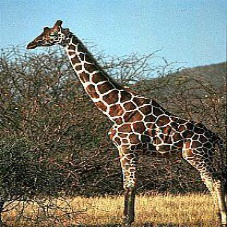
\includegraphics[width=2.5cm]{fig/giraffe_real.jpg}};
\node[font=\bfseries\Large] at ($(d2.south)!0!(d2.south)+(0,-1.5mm)$) {$\vdots$};
\node[rectangle, rounded corners=5pt, draw=blue, line width=1.5pt, below=5mm of d2,label={[font=\bfseries\Large]left:Domain N}] (d3) {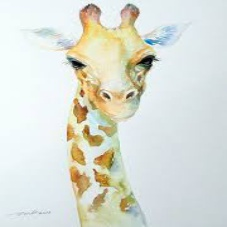
\includegraphics[width=2.5cm]{fig/giraffe_watercolor.png}};
% --- END OF MODIFICATION ---

\node[extractor, right=25mm of d2] (fe) {Feature \\ Extractor \\ ($F_\theta$)};
\matrix (z) [feature_vector, right=10mm of fe] {
    |[fill=z_cell_blue]| \\ |[fill=z_cell_yellow]| \\ |[fill=z_cell_blue]| \\
    |[fill=z_cell_blue]| \\ |[fill=z_cell_yellow]| \\ |[fill=z_cell_blue]| \\
    |[fill=z_cell_blue]| \\ |[fill=z_cell_yellow]| \\ |[fill=z_cell_blue]| \\ 
    |[fill=z_cell_blue]| \\  
};

\node[triangle_block, fill=classcolor, right=of z, yshift=3.5cm] (classifier) {Classifier \\ ($C_\psi$)};
\node[lossbox, xshift=2cm, right=of classifier] (loss_cls) {\bfseries\large $L_{\text{cls}}$};
\node[inputbox, above=5mm of loss_cls] (labels) {Labels Y};

\node[circle_block, fill=aligncolor, right=of z, yshift=-3.5cm] (l2norm) {L2 \\ Norm};
\node[lossbox, right=of l2norm, minimum width=5.5cm, minimum height=6cm] (loss_ot) {
    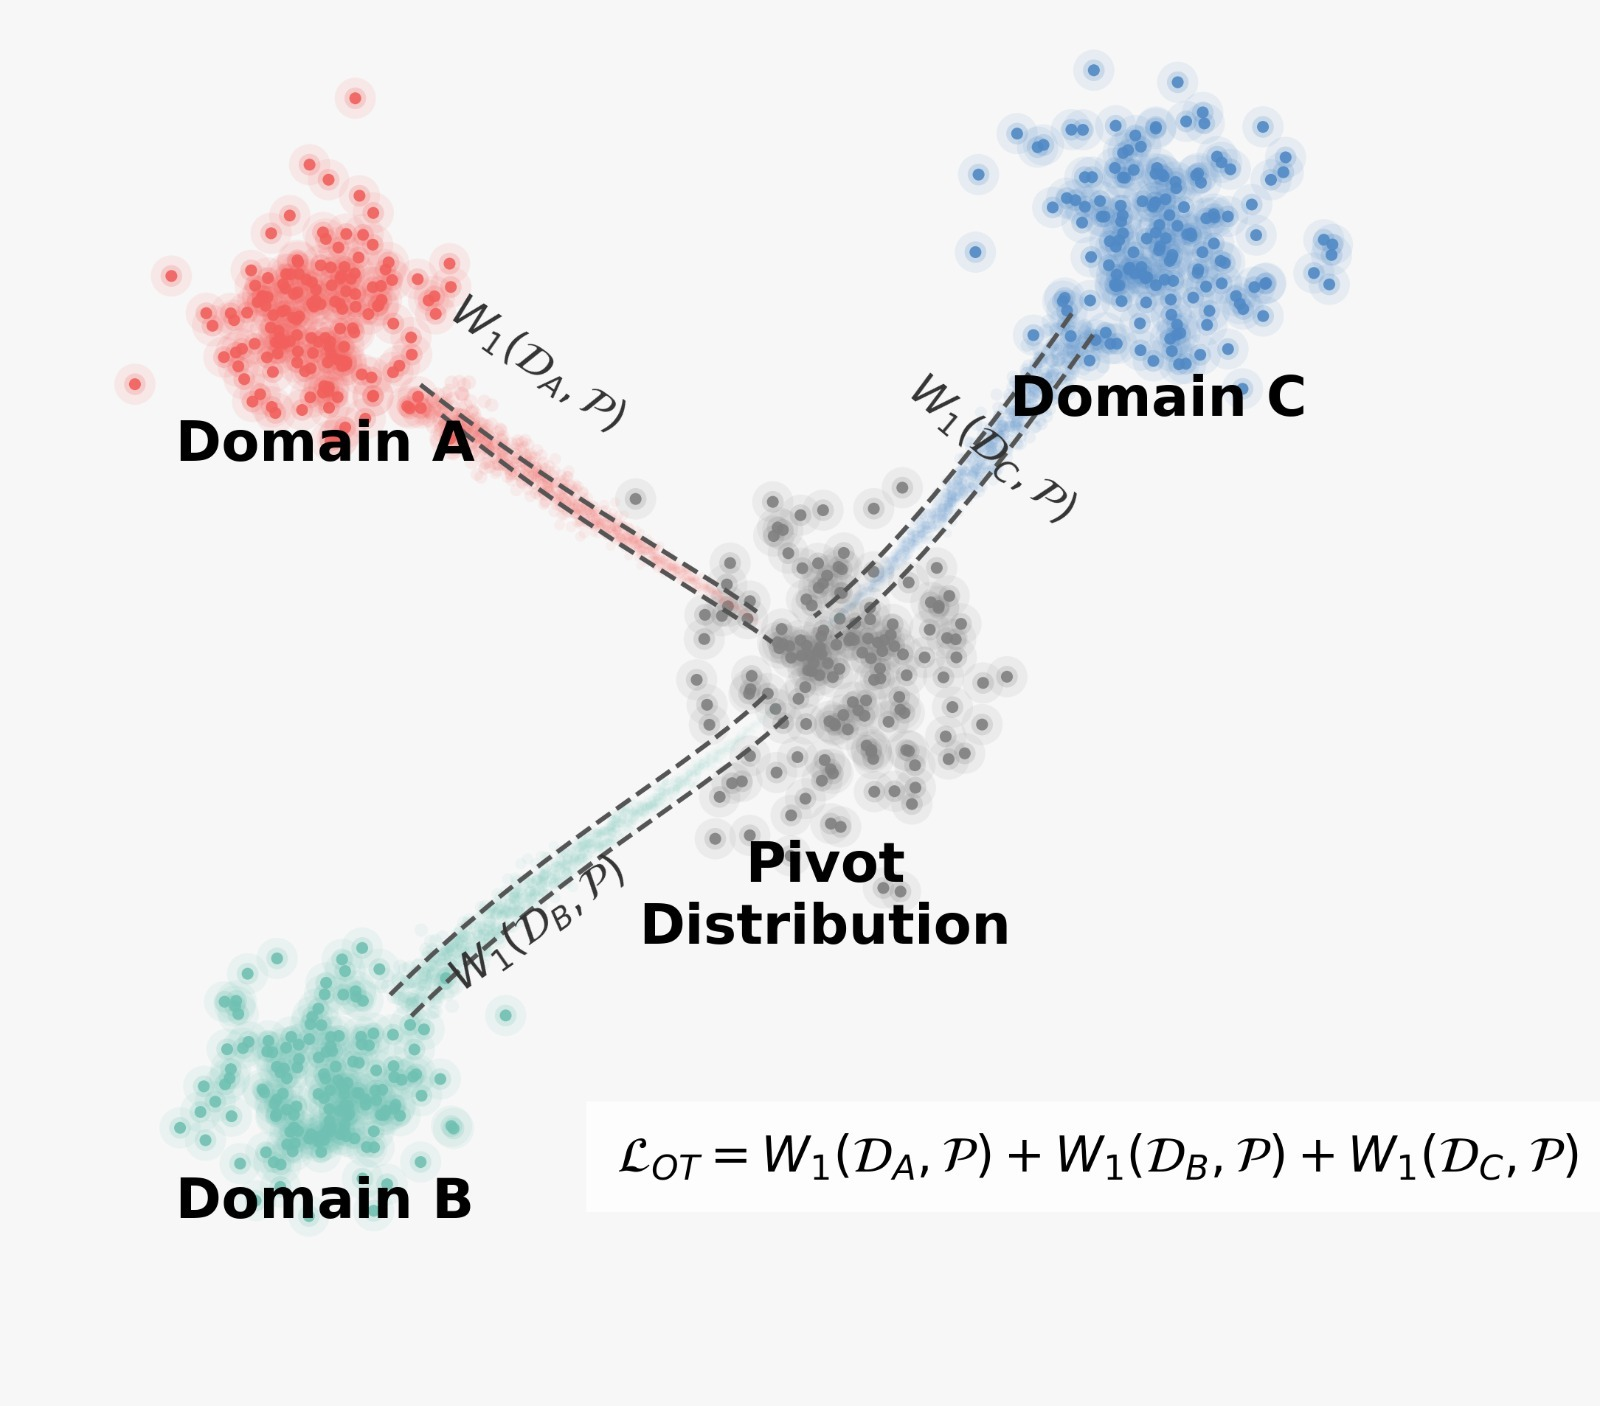
\includegraphics[width=11cm]{fig/ot_loss_plot.png} \\
    \vspace{2mm}
    \bfseries\large $L_{\text{OT}}$
};

\matrix (dfr_matrix) [matrix of nodes, below=of loss_ot, row sep=1.5pt] {
    |[dfr_cell, fill=dfr_item_blue]| \\
    |[dfr_cell, fill=dfr_item_green]| \\
    |[dfr_cell, fill=dfr_item_red]| \\
    |[dfr_cell_empty]| \\
    |[dfr_cell_empty]| \\
};
\node[fit=(dfr_matrix), draw=dfrborder, line width=1.2pt, rounded corners=3pt, inner sep=3pt] (dfr) {};
\node[below=2pt of dfr, align=center] {
      \bfseries\Large Dynamic Feature Reservoir (DFR) \\ \Large $Q \in \mathbb{R}^{K \times d}$
};

\node[totalbox, right=of loss_ot, xshift=2cm, yshift=1.5cm] (loss_total) {
    \bfseries\large $L_{\text{Total}}$ \\ \mdseries\Large $= L_{\text{cls}} + \lambda L_{\text{OT}}$
};

% == 4. DRAW ARROWS AND CONNECTIONS ==

\draw[arrowstyle, draw=black!70] (d1.east) -- (fe.west);
\draw[arrowstyle, draw=black!70] (d2.east) -- (fe.west);
\draw[arrowstyle, draw=black!70] (d3.east) -- (fe.west);
\draw[arrowstyle, draw=arrowmain] (fe.east) -- (z.west) node[midway, above, font=\bfseries\color{arrowmain}] {Z};

\coordinate (z_split_point) at ($(z.east)$);

\draw[arrowstyle, draw=arrowclass] (z_split_point) to[out=45, in=180] (classifier.west);
\draw[arrowstyle, draw=arrowalign] (z_split_point) to[out=-45, in=180] (l2norm.west);

\draw[arrowstyle, draw=arrowclass] (classifier.east) -- (loss_cls.west);
\draw[arrowstyle, draw=arrowclass] (labels.south) -- (loss_cls.north);
\draw[arrowstyle, draw=arrowalign] (l2norm.east) -- (loss_ot.west);

\draw[arrowstyle, draw=dfrborder, line width=1.5pt] (dfr.north) -- (loss_ot.south) node[midway, right, font=\small]{Read};
\draw[arrowstyle, draw=arrowalign, dashed] (l2norm.south) |- (dfr.west) node[midway, above right, font=\small]{Update};

\draw[arrowstyle, draw=black!60] (loss_cls.east) to[out=0, in=140] (loss_total.west);
\draw[arrowstyle, draw=black!60] (loss_ot.east) to[out=0, in=220] (loss_total.west);

\draw[arrowstyle, draw=backproppink, dashed] (loss_total.north) to[out=90, in=0] ($(loss_total.north) + (-6cm,10cm)$) to[out=180, in=90] ($(fe.north) + (0,1cm)$) to[out=270, in=90] (fe.north);

% == 5. LEGEND ==
\begin{scope}[node distance=2mm, font=\sffamily\small, text=black,
              every node/.style={anchor=west}]
    \node[draw=black!40, fill=white, rounded corners=5pt,
          left=of dfr, xshift=-10cm, align=left] (legend_box) {
        \begin{tabular}{p{1.5cm} l}
            \tikz\draw[arrowstyle, draw=arrowclass] (0,0) -- (1,0); & Classification path \\
            \tikz\draw[arrowstyle, draw=arrowalign] (0,0) -- (1,0); & Alignment path \\
            \tikz\draw[arrowstyle, draw=arrowalign, dashed] (0,0) -- (1,0); & Update (no gradients) \\
            \tikz\draw[arrowstyle, draw=backproppink, dashed] (0,0) -- (1,0); & Backpropagation \\
            \tikz\draw[arrowstyle, draw=dfrborder] (0,0) -- (1,0); & DFR read operation \\
        \end{tabular}
    };
\end{scope}

\end{tikzpicture}
} % End of resizebox
\caption{Overview of SODA. The framework consists of a standard supervised path (\textcolor{blue}{blue}) and a stabilized OT alignment path (\textcolor{purple}{purple}). Crucially, the Dynamic Feature Reservoir (DFR) is updated via a gradient-free queue mechanism (dashed line), ensuring it acts as a stable anchor. The alignment loss $\mathcal{L}_{OT}$ minimizes the entropic OT cost between the current mini-batch features and the non-parametric distribution defined by the reservoir.}
\label{fig:soda_framework}    
\end{figure*}